\documentclass[10pt]{article}

\usepackage{amsmath}
\usepackage{graphicx}
\usepackage{epsfig}

\begin{document}

\title{Dispatch Module Document\\maTHmU }
\author{Wenlei Zhu}
\maketitle


\section{Overview}

\begin{itemize}
\item Dispatchers work as a load balancer or reverse proxy for our computing server nodes. 

\item dispatcher has the ability to connect to other dispatchers thus a dispatcher network can be built.
\end{itemize}

\section{illustration}
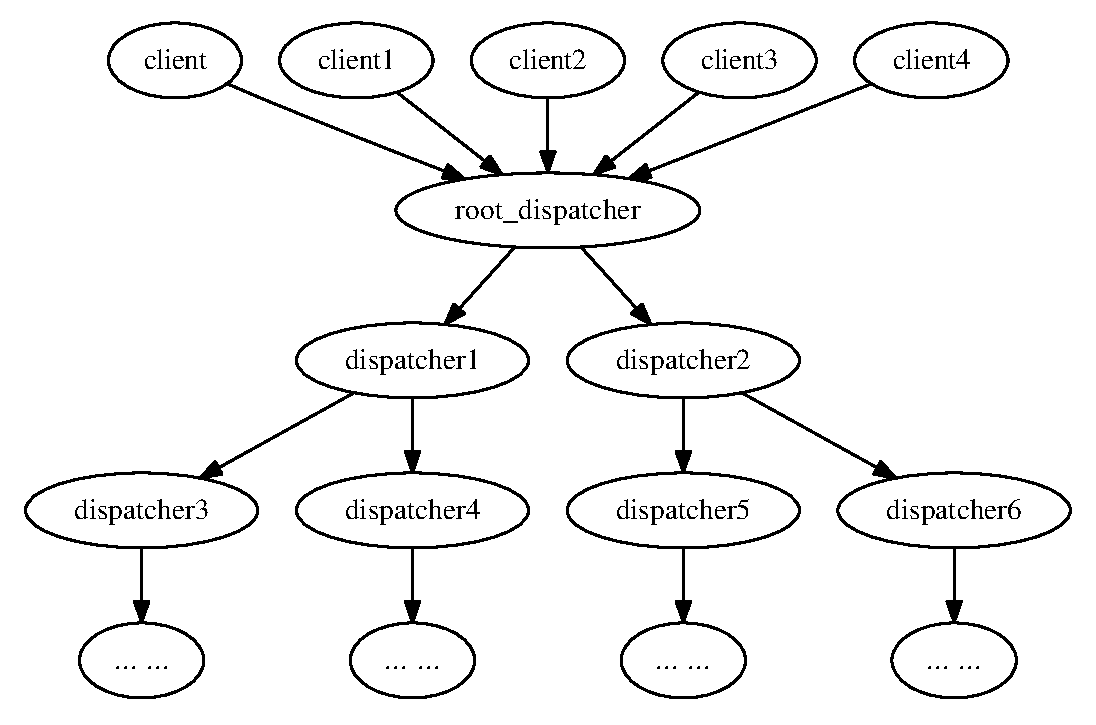
\epsfig{file=dispatch.eps,width=\linewidth}

\section{Details}
\begin{itemize}
\item When requests from clients come, they will be handled by dispatchers first, dispatchers then send these requests to other dispatchers or computing nodes according to the network structure. All the request will be sent to computing nodes, and corresponding results will be sent back through the dispatcher network to the client and presented properly.

\item Dispatchers manage context for clients, for that users need to execute context-related commands.For example, a user can define a variable in one command and use this variable in another command.

\item Every dispatcher manages a context table which stores the route for all the client through him. When new client request received, dispatcher will search the context table first, if client found, send the request to the next node according to the table, if client not found, select a route for this client using a specified algorithm and insert a new route item for this client to the context table. In this way, client session can be stored. And we can send a client’s requests to the same computing node.

\item As mentioned above, when a client’s first request goes through a dispatcher, the dispatcher will choose a path for it. So dispatchers control the network route. Thus we can do some control using dispatcher, for example, we can choose a fast computing node for a VIP user and a normal one for normal users.
\end{itemize}

\section{Node Operation}
The Dispatch module's server part also accept node operation commands, these commands begin with "node", 
provide the operation description to let the node manage its downstream node(maybe another dispatch node
or the actual computing node). The operation works only for the object we connected to, it will not 
dispatched to its children node as calculation tasks.

\subsection{description}
In the following commands,\\
$<ip>$ means an dotted decimal IP address representation.\\
$<port>$ means a interger represented port number on which the node server serves.
$[sth]$ means something optional\\
$|$ means OR 

\subsection{add node}
\subsubsection{description}
Add a calculation node to this dispatch module. The node can be another dispatch module or an actual 
calculation node.

\subsubsection{semantic}
\begin{verbatim}
node add <ip> [<port>]
\end{verbatim}
The default port is 5009 if port is not provided.

\subsubsection{example}
\begin{verbatim}
node add 192.168.1.101 5009
node add 192.168.1.102
\end{verbatim}

\subsection{remove node}
\subsubsection{description}
Remove a calculation node for this dispatch module. The operation will not take effect if the node 
dose not exists.[not implemented yet]

\subsubsection{semantic}
\begin{verbatim}
node [rm|del] <ip> [<port>]
\end{verbatim}
The default port is 5009 if port is not provided.

\subsubsection{example}
\begin{verbatim}
node del 192.168.1.101 5009
node rm 192.168.1.102
\end{verbatim}


\subsection{pause node}
\subsubsection{description}
Pause a calculation node for this dispatch module. The operation will not take effect if the node 
dose not exists.[not implemented yet]

\subsubsection{semantic}
\begin{verbatim}
node [stop|pause] <ip> [<port>]
\end{verbatim}
The default port is 5009 if port is not provided.

\subsubsection{example}
\begin{verbatim}
node pause 192.168.1.101 5009
node stop 192.168.1.111
\end{verbatim}

\subsection{resume node}
\subsubsection{description}
Resume a calculation node for this dispatch module. The operation will not take effect if the node 
dose not exists or not paused at all.[not implemented yet]

\subsubsection{semantic}
\begin{verbatim}
node resume <ip> [<port>]
\end{verbatim}
The default port is 5009 if port is not provided.

\subsubsection{example}
\begin{verbatim}
node resume 192.168.1.101 5009
\end{verbatim}

\subsection{list node}
\subsubsection{description}
Resume a calculation node for this dispatch module. The operation will not take effect if the node 
dose not exists or not paused at all.[not implemented yet]

\subsubsection{semantic}
\begin{verbatim}
node list
\end{verbatim}

\subsubsection{example}
\begin{verbatim}
node list
\end{verbatim}

\subsection{other ideas}
restart a node\\
increase weight\\
VIP route\\

\end{document}

